\chapter{Introduction}

The practice of staining glass for decorative purposes dates to ancient Rome,
but the investigation of light matter interaction starts even back to the
begining of history for human beings, when ancient men wondered about the
source of light ,sun, or the first time to use a torch for hunting. People
never stop studying how the light interacts with our world, meanwhile, this
leads to improving our understanding and building a better world with photonic
technology. The stained-glass windows such as the one inside of the St.
Patrick's Cathedral in Fig.~\ref{StainGlass} served as a 'poor man's Bible' in
the Middle Ages, allowing believers who could not read Latin to learn the story
of the Gospels.  The term stained glass refers to glass that has been coloured
by adding metallic salts during its manufacture. Then this coloured glass is
crafted into stained glass windows in which small pieces of glass are arranged
to form patterns or pictures. Even nowadays, people are still surprised about
how beautiful they are and wondering how the light interact with these pieces
of art crafts. Besides the arts, lighting technology is also evolving very
rapidly, from the ancient torchs to the bulb that Thomas Edison invented and to
the modern LEDs such as the ones also shown in Fig.~\ref{StainGlass}. From
blackbody radiation to electroluminescence, i.e., from thermal radiation to
radiative recombination, we are now capable of generating light more
efficiently.

\begin{figure}
  \caption{The Stained-glass window and the top modern lamps inside of the St. Patrick's Cathedral, 5th Ave, New York, NY.}
  \centering
  
\includegraphics[width=0.5\textwidth,height=0.5\textheight]{pictures/Introduction/StainGlass}
  \label{StainGlass}
\end{figure}

Now we find ourselves living through a new revolution in the age of information
technology, one with consequences every bit as dramatic and likely even more
profound as the data transmission by light. Electrons have served us very well
for the past few decades, but the explosion of data. The storage and the
transmission of data consumes large amount of power and time, simultaneously.
Meeting the energy needs of the communication of information, together with
storage and computation form a "grand challenge" of the information age.

One good example of huge amount of power consumption by data transmission and
computation is the data centers, which currently consume 1.5\% of global energy
production, and up to approximately 4\% of U.S. energy produced. Though the
statistics seems small, a 1000 times increase in the volume of data is
predicted by 2025~\cite{Hilbert:2011tg}. Google data center alone consumes
enough electricity to power 200,000 homes, since an average Google search or a
YouTube video or a message through Gmail uses 0.3 watt-hours of
electricity~\cite{glanz2011google}. Having efficient data computation and
transmission tools will greatly reduce the total data center power consumption
into a greener number. And the data pipelines of light can certainly be very
helpful in this regime.

\section{Background} \label{sec:intro_BG}

\subsection{Photonics and Optoelectronics}

Photonics involves the generation, control and detection of lightwaves and
photons, which are particles of light, in free space or solid.
Optoelectronics is the study and application of effects related to the
interaction of light and electronic signals, and may be considered a sub-field
of photonics. Both photonics and optoelectronics study the light, and explore a
wider variety of wavelengths besides visible lightwave range, from gamma rays
to radio, including X-rays, ultraviolet and infrared light.

The invention and development of solar
cells~\cite{sun2005organic,perlin1999space},
photodetector~\cite{razeghi1996semiconductor,rogalski2002infrared},
modulators~\cite{chen2011broadband,schuller2010plasmonics},
LEDs~\cite{spanggaard2004brief,schubert2005solid,schubert2005light} and
lasers~\cite{chow2012semiconductor,yablonovitch1987inhibited} certainly set the
example of breakthroughs due to the manipulation of photons in thin films and
semiconductor bulk crystals. The continuing success of photonic technologies
relies on the discovery of new optical materials and the miniaturization of
optoelectronic devices that feature better performance, low cost and low power
consumption. For the last few decades, countless efforts in nano-scale
materials and devices research have created a rich collection of nanostructures
where size, shape and composition can be readily controled. Many such
nanostructures exhibit fascinating optical properties that could have
significant impact in the future for photonic technology.

\subsection{Core-Shell Nanowires} \label{sec:intro_CSNW}

The primary principle for constantly miniaturizing the device is not only about
the size, but also to have better electronic and optical properties. As the
critical dimension of semiconductor solid-state devices keep shrinking, the
effect of charge carriers quantization becomes more prominent, and to be more
specific, this means the confinement of electrons or holes by constructing
quantum confined structures. At the very dawn of electronics, the idea of using
heterostructures (i.e., the structure with two layers or regions of dissimilar
crystalline semiconductors) has emerged. After Shockley proposed the idea,
Alferov and Kroemer introduced the concept that heterojuctions could possess
high injection efficiencies in comparison with homojunctions, and which we know
now is due to the confinement of carriers~\cite{alferov2000double}. It would be
very difficult today to imagine solid-state physics without semiconductor
heterostructures for both electronic-based and optical-based applications. The
heterostructures and, especially, double heterostructures, including quantum
wells, nanowires, and quantum dots, are the fundamental building blocks for
current nanoscience research as depicted in Fig.~\ref{Nanomaterials}.

\begin{figure}
  \caption{Diagram of classification of nano-materials and nano-scale structures}
  \centering
  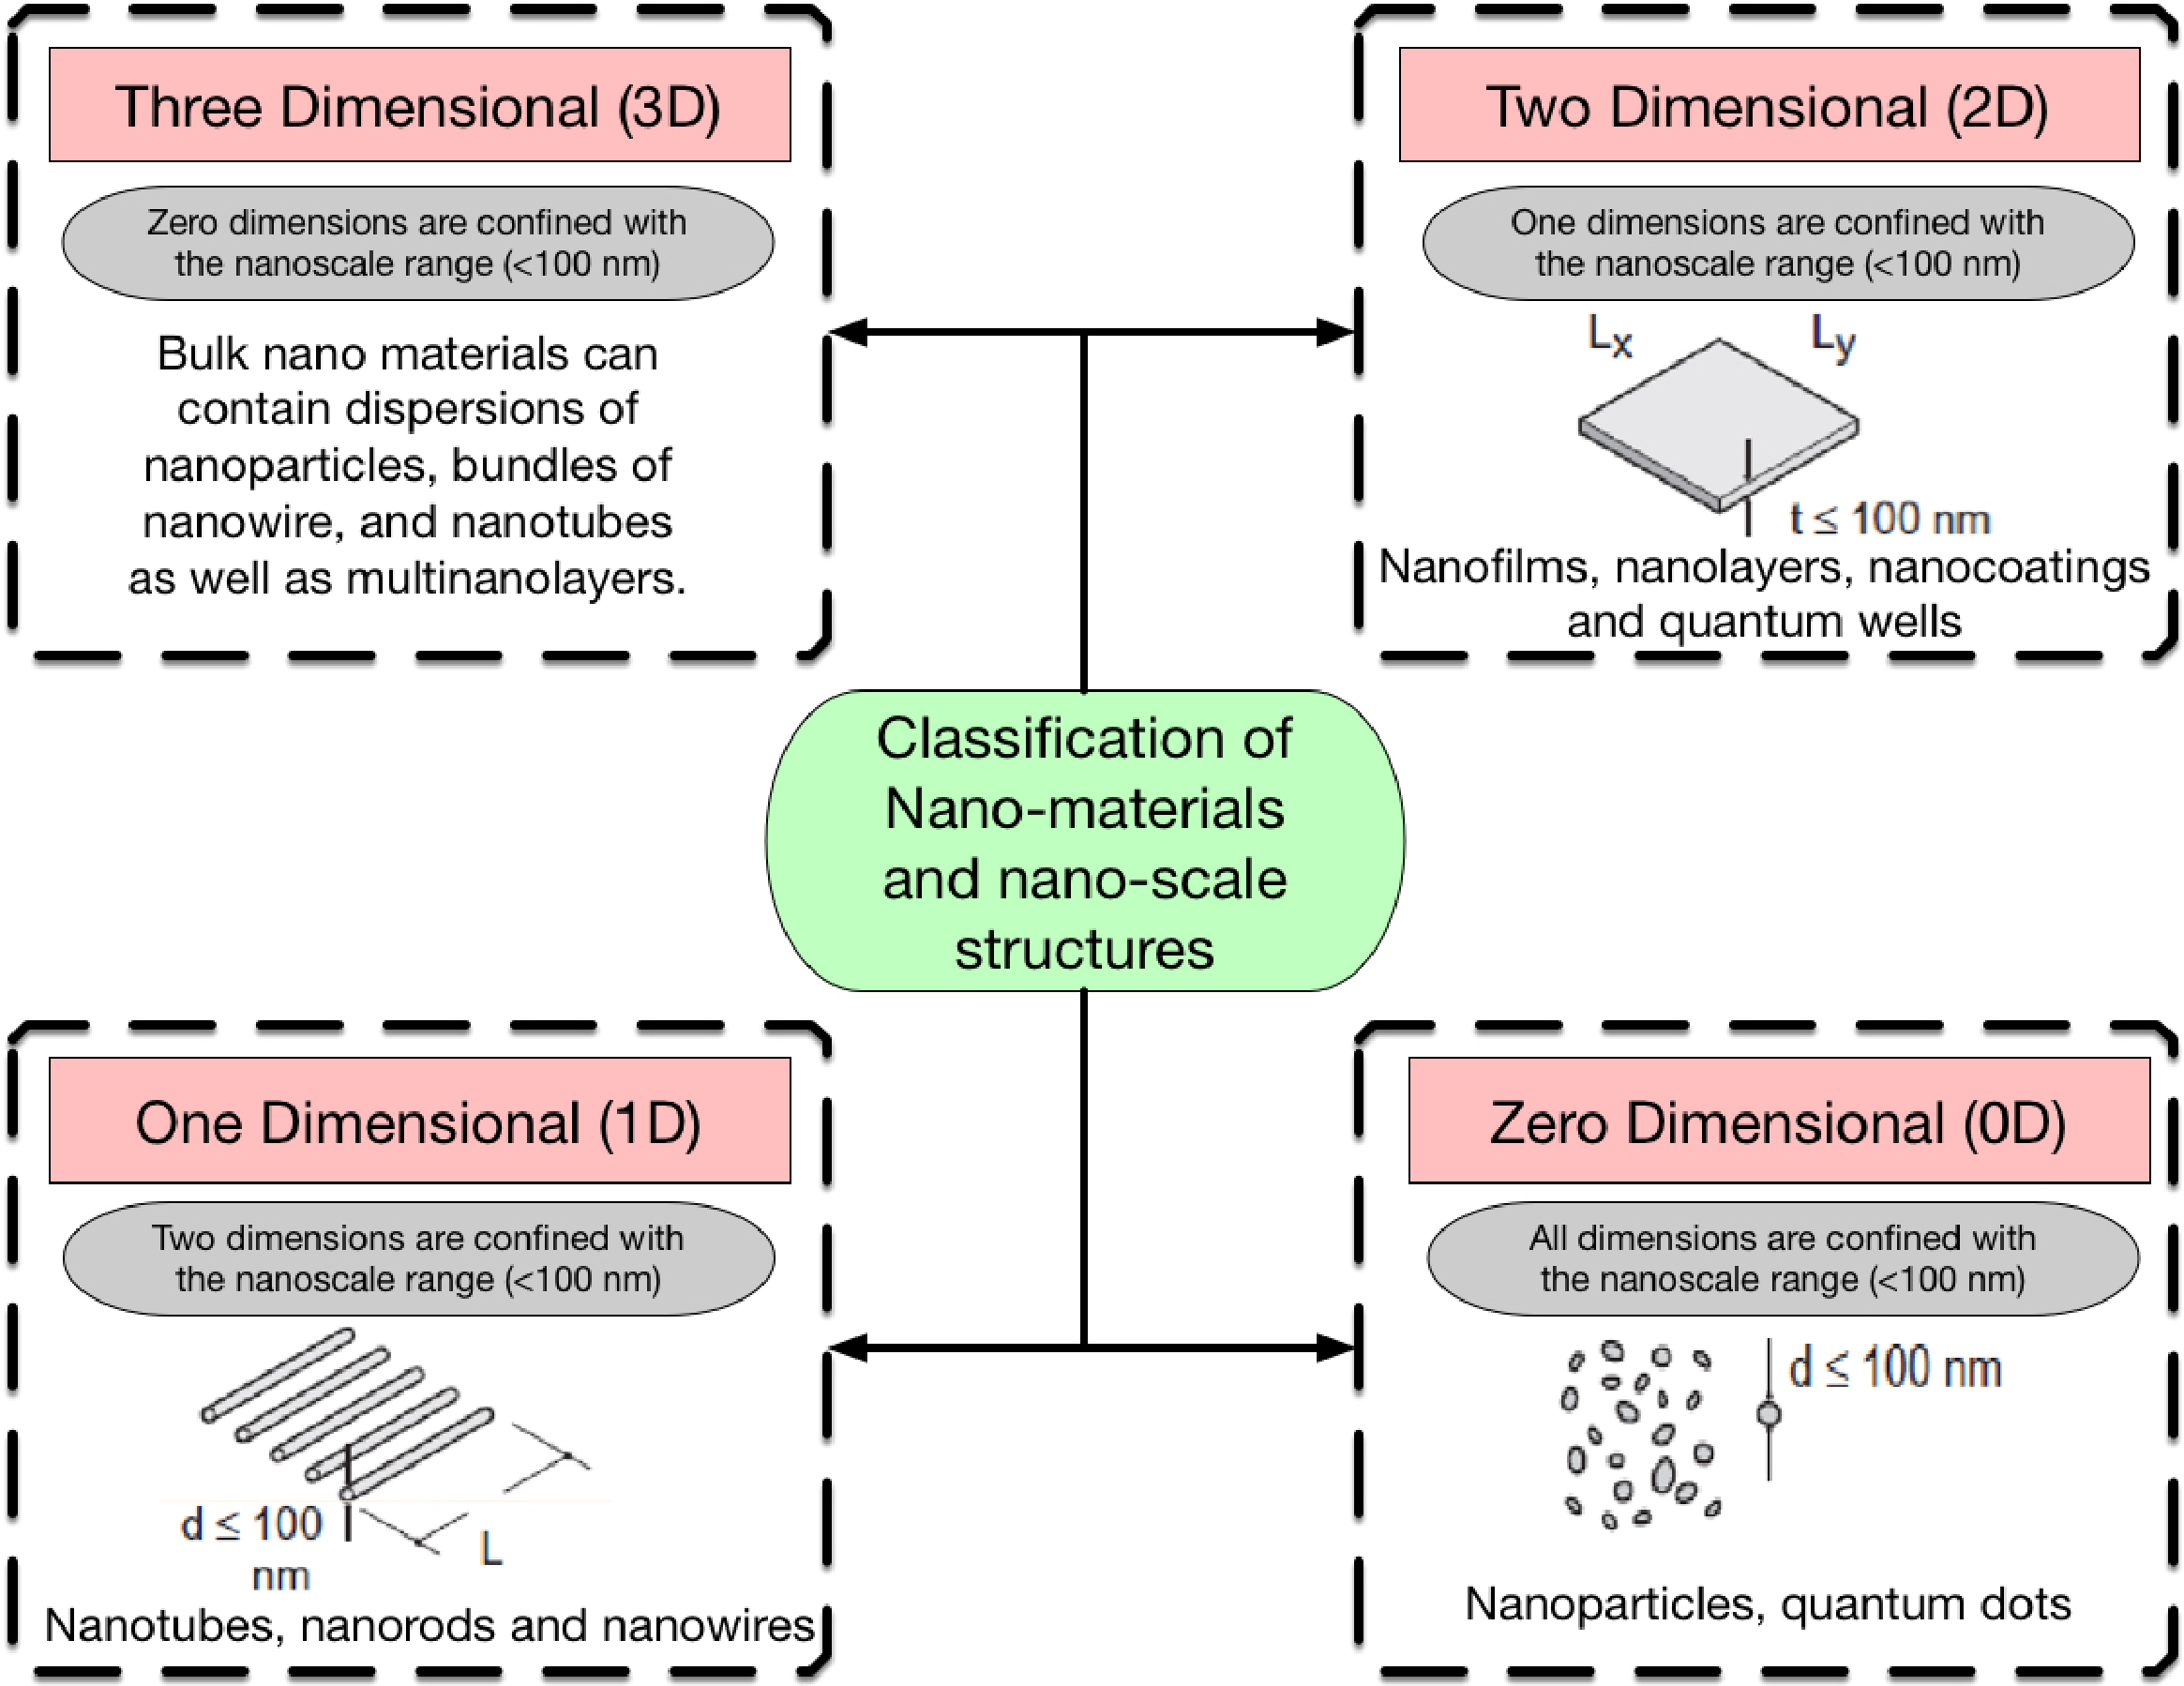
\includegraphics[width=\textwidth]{pictures/Introduction/Nanomaterials}
  \label{Nanomaterials}
\end{figure}

Quantum well is a potential well which confines particles to only move freely
in two dimensions in stead of three dimensions, by forcing them to occupy a
planar region. These wells are typically formed in semiconductors by having a
narrower bandgap material sandwiched between two layers with wider bandgap
materials. Electrons in quantum wells are confined in two dimensions either
naturally or by doping the barrier of a quantum well, thus a two-dimensional
electron gas (2DEG) may be formed at the heterointerface. This not only
increases the density of electrons, but also causes a better performance in
optoelectronic devices such as laser diodes~\cite{nakamura1996ingan}, High
Electron Mobility Transistors (HEMTs)~\cite{kuzmik2002inaln,rosenberg19850},
photodetectors~\cite{levine1993quantum,liu2004terahertz}, and solar
cells~\cite{barnham2002quantum,ekins1999strain}.

Quantum dots, as another most common nanostructure in semiconductor physics,
exhibit much more enhanced optical properties. They are normally only several
nano-meters in size, and either synthesized or self-assembled into a bulk
solid. As the particles in the quantum dots are confined in three dimensions,
which leave them zero degree of freedom. As a result, the density of states
changes to a delta function as opposed to a smooth square root dependence that
is found in bulk materials. The narrower peak spectra and larger magnitude of
intensity make them even better candidates in the application of solar
cells~\cite{nozik2002quantum},
lasers~\cite{klimov2000optical,ustinov2003quantum} and light emitting diodes
(LEDs)~\cite{park2001band,sun2007bright}.

However, since the introduction in the 1990's, another important class of
semiconductor nanostructures has emerged: structures with cross-sections of
tens or hundreds of nano-meters and lengths up to several micro-meters. These
structures are named as 'nanowires'~\cite{xia2003one} different from quantum
dots as they are confined only in two dimensions, thus allowing electrons,
holes or photons to propagate freely along the third dimension. Besides their
own outstanding electro-optical properties, the high-aspect-ratio of these new
semiconductor nanostructures allows for the bridging of the nanoscopic and
macroscopic world. As P. Yang writes in their review paper:~\cite{Yan:2009hm}
"This nano-macro interface is fundamental to the integration of nanoscale
building blocks in electrical or optoelectronic device applications.
Conventional photonic platforms often consist of features with large
aspect-ratios such as interconnects and waveguides, typically with micrometre
dimensions. Thus, when semiconductor nanowires emerged they were immediately
recognized as one of the essential building blocks for nanophotonics."

The development of sophisticated nanowires growth
techniques~\cite{hobbs2012semiconductor,wu2001direct}, either
bottom-up~\cite{lu2007nanoelectronics,Huang:2001kv} or
top-down~\cite{park2009top}, has stimulated a large body of new work in
semiconductor nanowires over the last twenty years or so. Previously, the
research activities focused on the growth of higher quality
nanowires~\cite{Yang:2002ts} and the variation of its constituent materials. At
that time, most of the nanowires were core-only with ZnO~\cite{Yang:2002ts},
GaAs~\cite{persson2004solid}, Si~\cite{hochbaum2005controlled}, or
Ge~\cite{wu2000germanium}. However, later on, researchers found out that
growing an additional layer of shell can increase quantum yield by passivating
the surface trap states. In addition, the shell provides protection against
environmental changes, photo-oxidative degradation, and provides another route
for modularity. Precise control of the size, shape and composition of both the
core and the shell enable engineering the device with many degree of freedom
and optoelectronic properties, such as the tuning of the emission wavelength
over a wider range of wavelengths than with either individual semiconductor.
Undoubtedly, much of this interest was further stimulated by the possibility of
novel physics and applications in core-shell nanowires.

The successes of semiconductor nanowires in optoelectronics and the promising
physical mechanisms using quantum-confined structures have, furthermore,
enlivened the debate over possible applications of optics for functions such as
transmission, logic and switching in communications and computation. It is
important to emphasize at the outset that quantum confinement produces not only
quantitative but also qualitative differences in physics compared to that in
bulk structures, which is of course another major motivation for the interest
in them. As Dr. Miller discussed in the paper about quantum
well:~\cite{schmitt1989linear} "There are many examples of these differences.
The optical absorption spectrum breaks up into a series of steps associated
with the quantum-confined electron and hole levels. Excitonic effects become
much stronger because of the quantum confinement, giving clear absorption
resonances even at room temperature. The relative importance of direct Coulomb
screening and exchange effects is quite different in quantum wells (the Coulomb
screening is relatively much weaker), giving very different optical saturation
behaviour." Similar to quantum wells, nanowires have been observed to have even
more profound differences in physics. Thus, the analysis and discussion about
different behavior of nanowires and bulk semiconductors when they interact with
light will be the primary topic of this dissertation.

\section{Literature Review} \label{sec:intro_LR}

Since the introduction of initially so-called 'nanowhiskers' in the
1990s~\cite{yazawa1991heteroepitaxial}, semiconductor nanowires have been
extensively studied and much insight has been gained on tuning their electrical
and optical properties. Nanowire related articles have shown a healthy increase
in number published from 2005 to 2016, as Fig.~\ref{ISIPublication} (blue bars)
shows. Article with topics on optical properties of nanowires comprise a good
portion in all the nanowire-related papers published in the recent decade,
showing clear increasing trend in the number of papers on NW optics or
photonics (green bars), presently comprising more than four-fifth of the
nanowire-related articles.

\begin{figure}
  \caption[Article with topics on optical properties of nanowires consist of a large portion of all the nanowire-related papers published from 2005 to 2016.]{Article with topics on optical properties of nanowires consist of a large portion of all the nanowire related papers published from 2005 to 2016. (Source: ISI website, keyword: Nanowire (blue), Nanowire AND optical OR optoelectronic OR photonics (grey))}
  \centering
  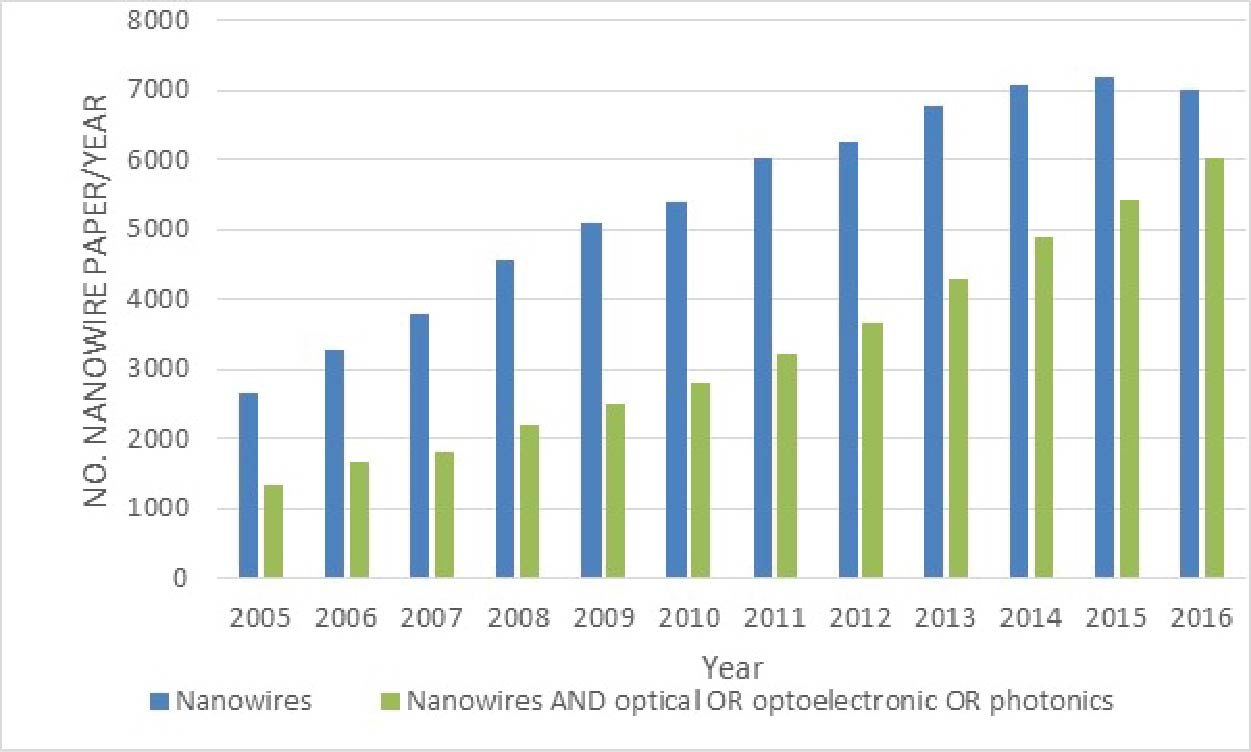
\includegraphics[width=\textwidth]{pictures/Introduction/ISIPublication}
  \label{ISIPublication}
\end{figure}

The applications and classifications of NWs are shown in
Fig.~\ref{NWApplication}. In terms of the geometric strcuture, the most common
NWs are cylindrical~\cite{Cao:2010dc,Cao:2009ho} and
hexagonal~\cite{Royo:2015vw,Currie:2013to} due to the growth techniques. And as
discussed previously, there are
core-only~\cite{Heo:2004fp,he2007piezoelectric,Duan:2003en},
core-shell~\cite{Moratis:2016ws,Wang:2015bz} and
core-multi-shell~\cite{Badada:2015jq,Takehiro:2016tl} configurations in order
to exploit various properties of NWs. In addition, NWs have been used as
electronic based devices, such as High Electron Movement Transistors
(HEMTs)~\cite{li2006dopant,sakaki1980scattering}, Field Effect Transistors
(FETs)~\cite{xiang2006ge,singh2006high,suk2005high},
capacitors~\cite{Liu:2012cz}, diodes~\cite{Wallentin:2010kf,heo2004pt},
and optoelectronic based devices, such as
lasers~\cite{Li:2015ir,Wei:2014hr,Saxena:2013fe,Mayer:2013jh,Chen:2011cg,Hua:2009kf,Agarwal:2005is,Gradecak:2005eb,Duan:2003en},
LEDs~\cite{Zhao:2015hl,Nami:2015df,Chuang:2011jk,Bavencove:2011io,Kim:2004je},
Solar Cells~\cite{Wang:2015dp,Yu:2014hj,Wang:2012dh,Kelzenberg:2010fa,Garnett:2008jk,Tsakalakos:2007kz,Tian:2007kl},
Photodetectors~\cite{Chen:2015dz,deLunaBugallo:2010ci,Cao:2010dc,Pettersson:2006ft,Kind:2002fk,Liang:2001ka},
waveguides~\cite{Grego:2011ka,Oulton:2008fi,Yamada:2005bl,Sirbuly:2005ir,Chandrasekhar:1987kk},
phototransistors~\cite{Zhang:2010fq,Seo:2010cf,Persano:2010if,Park:2008cn,Logeeswaran:2008fw}.

\begin{figure}
  \caption{Diagram of nanowires applications and classifications}
  \centering
  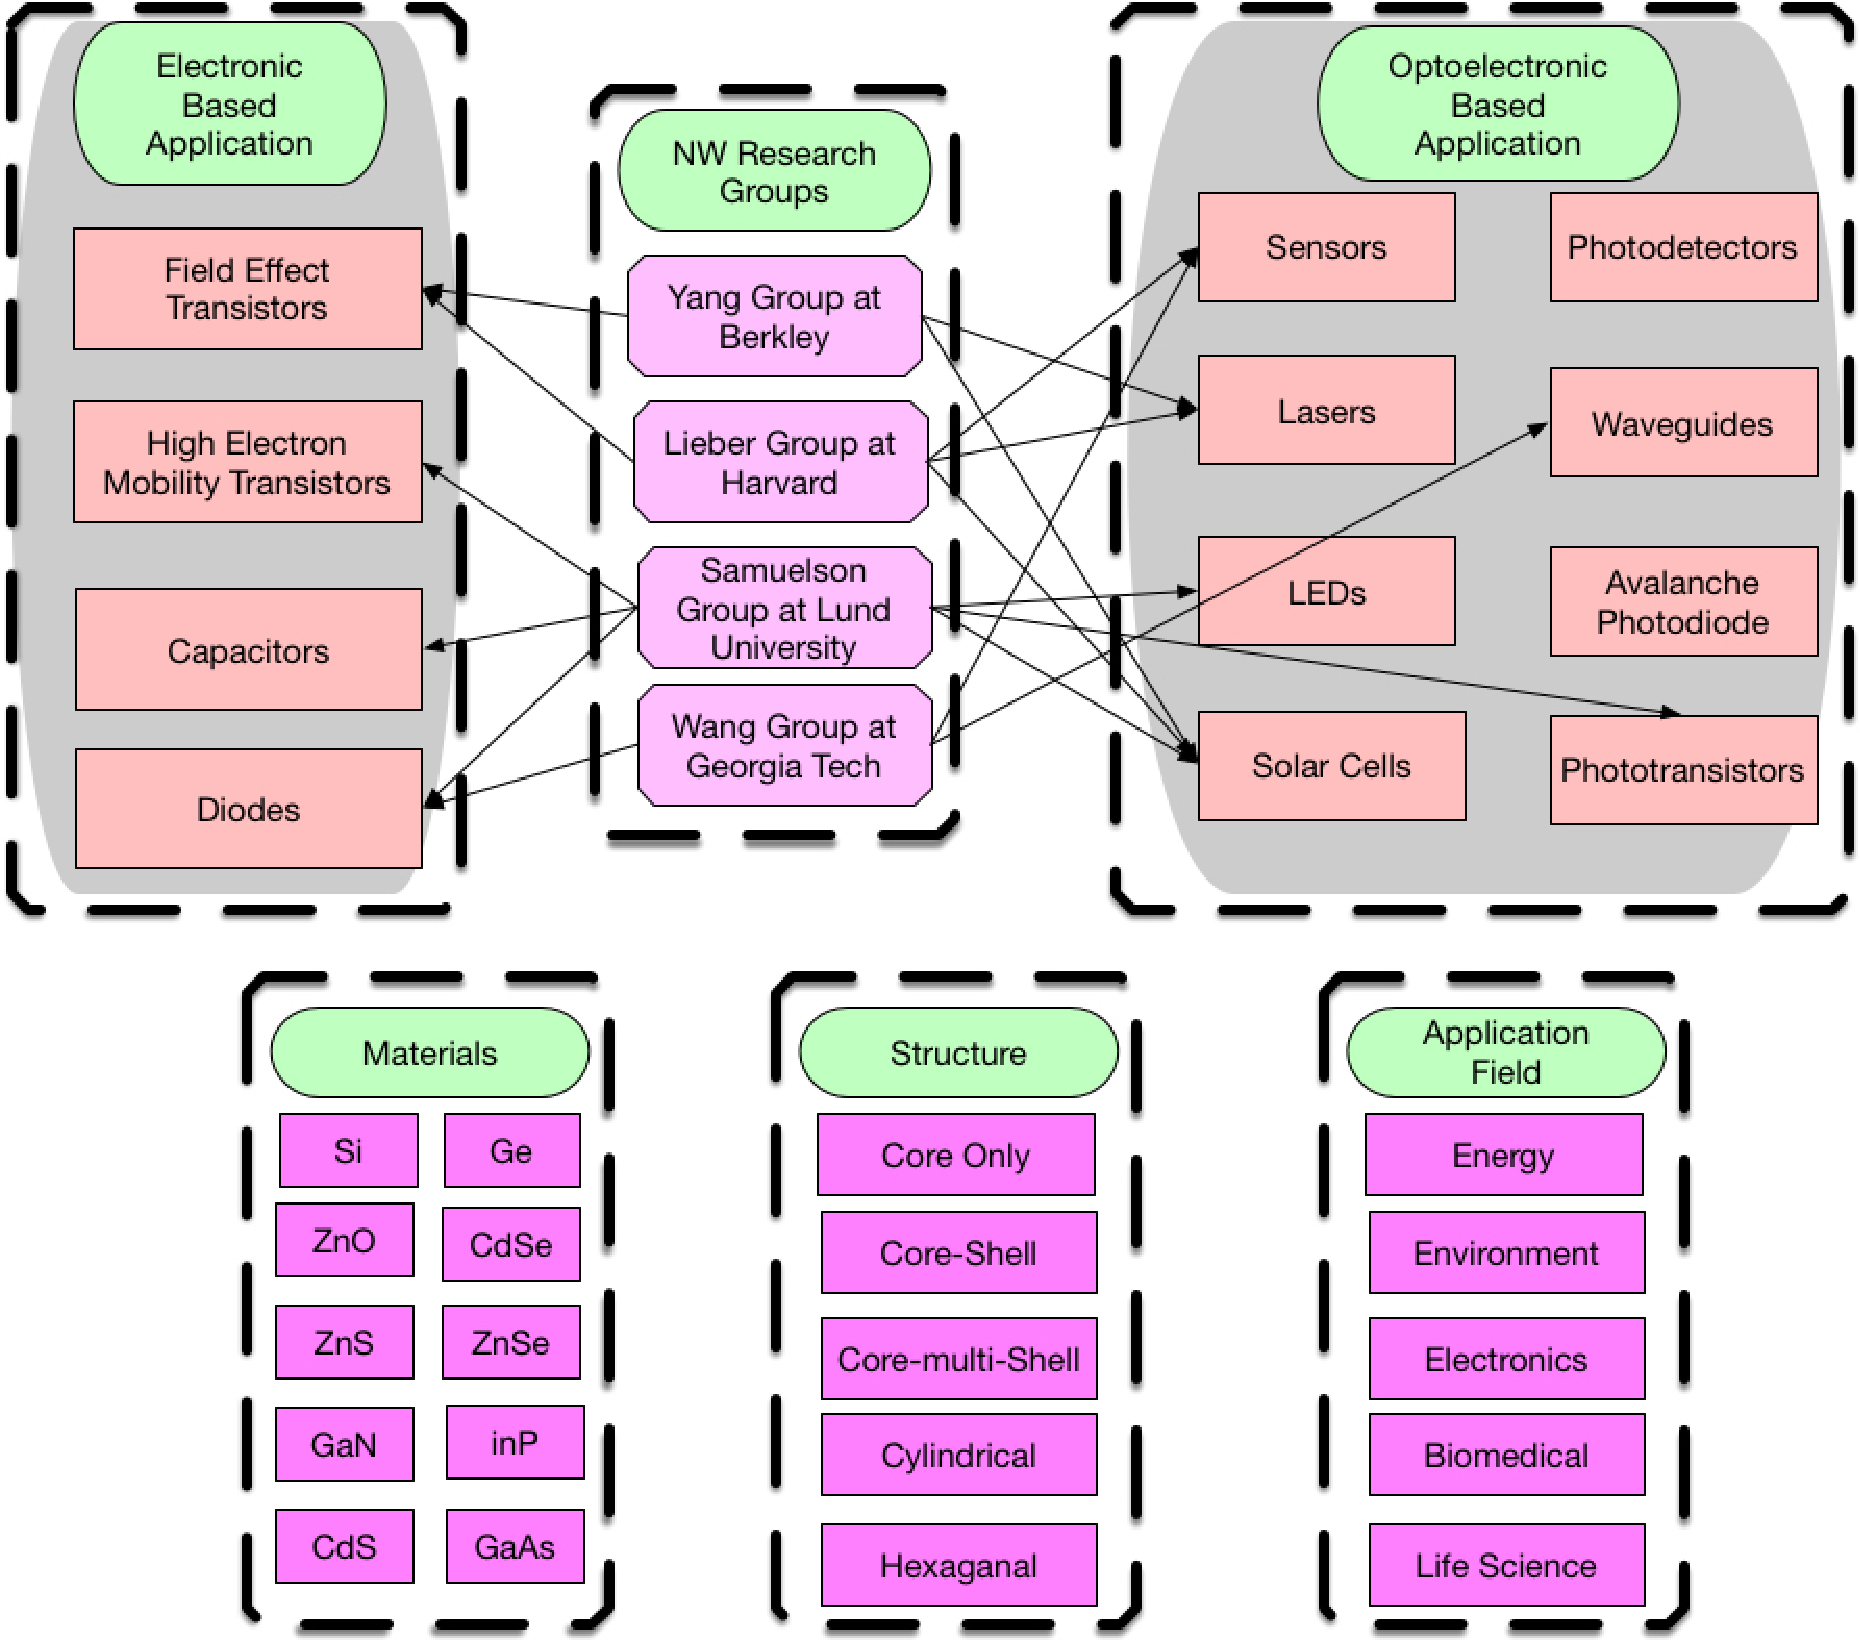
\includegraphics[width=\textwidth]{pictures/Introduction/NWApplication}
  \label{NWApplication}
\end{figure}


Exciting developments have been made in the academia environment from many
research groups worldwide, including notably the Lieber group at Harvard
University~\cite{Agarwal:2005is,Gradecak:2005eb,Patolsky:2005uz,Duan:2003en,li2006dopant,qian2008multi},
the Yang group at
Berkeley~\cite{Johnson:2003ww,Wu:2002ws,Kind:2002fk,Yang:2002ts,wu2001direct},
the Samuelson group at Lund
University~\cite{Ganjipour:2014cm,Storm:2012gm,Wallentin:2010kf,Thelander:2008uw,Pettersson:2006ft},
and the Wang group at Georgia
Tech~\cite{pan2001nanobelts,wang2006piezoelectric,wang2013nanowires,bae2011fiber,wang2007direct,he2007piezoelectric}.
With different perspectives, these research groups focus on a variation of NW
materials, growth techniques and applications as shown in
Fig.~\ref{NWApplication}. The development of semiconductor NW materials follow
the similar road as bulk materials, from initial single element (e.g.,
Si~\cite{hochbaum2005controlled}, Ge~\cite{wu2000germanium},
Carbon~\cite{zhao2003carbon} et al.) to compound binary
(ZnO~\cite{Johnson:2003ww}, GaN~\cite{Das:2011ci,Gradecak:2005eb},
CdSe~\cite{Persano:2010if}, ZnS~\cite{Ding:2004di}, ZnSe~\cite{xiang2003green},
InP~\cite{Logeeswaran:2008fw}, CdS~\cite{Ding:2004di}, GaAs~\cite{Joyce:2007bl}
et al.), ternary (InGaAs~\cite{Zhao:2014jt}, CdSSe~\cite{pan2006fabrication},
AlGaN~\cite{Li:2015ira}) or even quaternary (AlInGaN~\cite{Wang:2015bi}), then
to currently popular III-V heterostructure NWs(e.g.,
GaAs/AlGaAs~\cite{Peng:2014ia,Wei:2014ws}, GaAs/InGaAs~\cite{Chen:2011ct},
InGaN/GaN~\cite{Zhang:2016tk}, GaAs/GaAsP~\cite{Hua:2009kf} et al.). 

At the same time, many important electronic and optical properties have been
observed, and some of the fundamental applications have been demonstrated as
well. The first optical pumped nanowire laser was demonstrated by the Yang
group~\cite{Huang:2001kv} at 2001, and two years later, the Lieber group showed
the first electrically injected nanowire laser~\cite{Duan:2003en} which makes
NW a potential candidate to be integrated in the electronic-based integrated
circuits.

In the field of industry and commercialization, several companies have started
their adventure in the areas like energy, environment, bio-medicine etc., with
products that influencing our daily life. The glo-USA, Inc.~\cite{GloLED:2017}
is an LEDs manufacturing company at Sunnyvale, CA. They use nanowire arrays
which fabricated on chip to generate light as shown in Fig.~\ref{GloLED}(a).
Each nanowire acts basically as an individual light-emitting diode (LED) with
two circular metal contacts as anode and cathod. The inset is the 45 degree
magnified view of the NW array. Except the fabricated blue nLED as in
Fig.~\ref{GloLED}(b), all color of the visible spectrum, ranging from deep blue
to red, can be realized using nanowire LEDs with industry-standard
semiconductor material and manufacturing equipment.  Since these nanowires are
made using one material system with the active layers grown on the non-polar
plane, they can reduce the wavelength shift and efficiency drop that are
observed with other commercially-available planar LEDs. This will enable a true
white RGB (red, green and blue) LED without the need of lossy phosphor
conversion, thus achieving the highest Color Rendering Index (CRI) and
efficiency.

\begin{figure}
  \caption[Scanning Electron Microscopy image of actual glo nanowire chip and the fabricated blue nLED.]{(a) SEM of actual glo nanowire chip showing magnified 45 degree view of  individual nanowires. (b) The fabricated blue nLED. Each dot represents a nanowire LED. The inset shows top view SEM of nanowire array. Courtesy of glo-USA, Inc.}
  \centering
  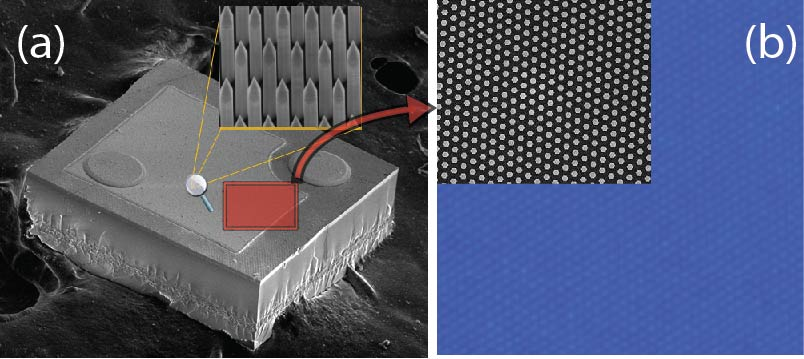
\includegraphics[width=\textwidth]{pictures/Introduction/GloLED}
  \label{GloLED}
\end{figure}

From academic research to industrial applications, from efficient electrons
transportation to high quality light confinement, and from applications for
environmental concerns to electronic devices in the daily life, the interaction of
light and nanowires need to be investigated, thus, the major topic of this
dissertation is to study the optoelectronics properties of core-shell nanowires
and how they interact with light when electrons in this nano-scale structure
are confined to lower dimensionality.

\section{Scope and Organization of the Dissertation}

This thesis is structured as follows. The growth techniques and electro-optical
properties of core-shell nanowires are presented in Chapter~\ref{data}.  After
introducing four different light confinement mechanisms, i.e., Leaky Mode
Resonance, Whispering Gallery Modes, Fabry-Perot Resonant Mode and Helical
Resonance Modes, Chapter~\ref{LM} presents our findings for a generalized
volumetric modes with light management of sub-wavelength cavities.
Chapter~\ref{ED} presents our methods and findings for calculating band-bending
and electronic distribution in both cylindrical and hexagonal core-shell
nanowire by solving Poisson-Schrodinger equations self-consistantly.  In
Chapter~\ref{RM}, we apply the inter-band optical transition rates study to
understand the extremely enhanced optical properties of hexagonal core-shell
nanowires, and identify three primary factors (overlap integral, oscillator
strength and joint optical density of states) which are strong function of
dimensionality. The quantum mechanical derivation based on perturbation theory
and Fermi's Golden Rule used in this chapter are outlined in more detail in
Appendix~\ref{ch:rates}. The modeling of lasing threshold based on the optical
transition rates in Chapter~\ref{LT} confirmed that our theoretical
explanation, analysis and calculation of optical properties of core-shell
nanowire have a very strong dependence on electron confinement. Finally, we
present our conclusions in Chapter~\ref{conclusions}.

Throughout this work we use the term  {\em nanowires} (NWs) to represent a
specific quantum confined structure with cross-sections of 2-300 nm and lengths
upwards of several micrometers. There are other research groups using terms
such as {\em nanopillars}, {\em nanotubes} or {\em quantum well wires} (QWRs)
to discuss the same nanostructures.
